!TEX root = main.tex
\renewcommand{\labelenumi}{\alph{enumi})}

\section*{Examen 1}

\begin{questions}
\question \textbf{1.5pts. c/u} Considera la siguiente expresi\'on regular: 
\begin{equation}
    a(b + ba)^{*} + a(a + ab)^{*}bb
\end{equation}

\begin{equation}
    \underbrace{\underbrace{a}_{\alpha_{0}}\overbrace{(\underbrace{b + ba}_{\alpha_{1}})^{*}}^{\alpha_{4}} + \underbrace{a}_{\alpha_{0}}\overbrace{(\underbrace{a + ab}_{\alpha_{2}})^{*}}^{\alpha_{5}}\underbrace{bb}_{\alpha_{3}}}_{\alpha_{6}}
\end{equation}


Versi\'on 1 
\begin{enumerate}
    \item Diseñar un AFN-$\epsilon$, M considerando el mismo lenguaje de $\alpha$ mediante el método de síntesis de
    Kleene (se pueden omitir algunas transiciones $\epsilon$).
    \begin{center}
        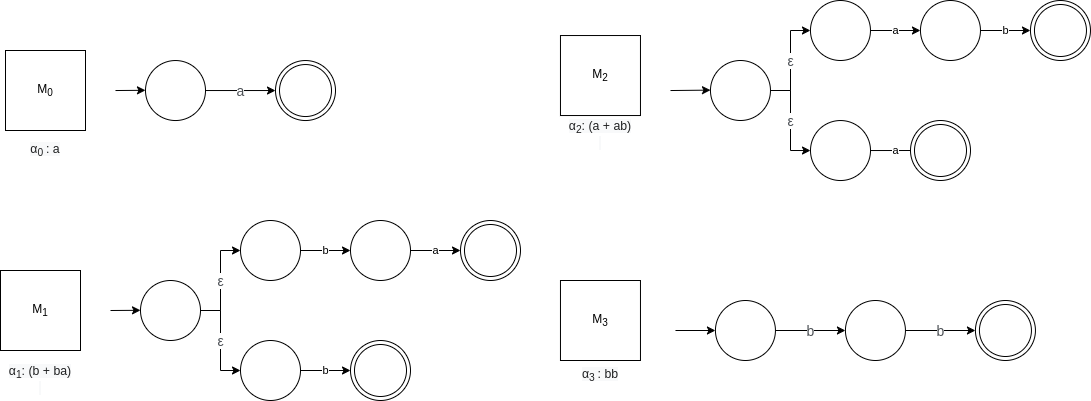
\includegraphics[scale=0.40]{exam3firstMachines.png}
        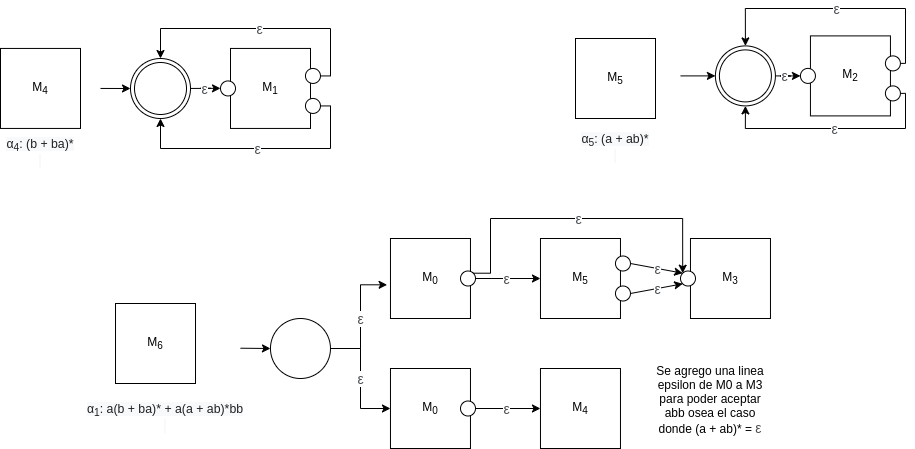
\includegraphics[scale=0.40]{exam3secondMachine.png}
        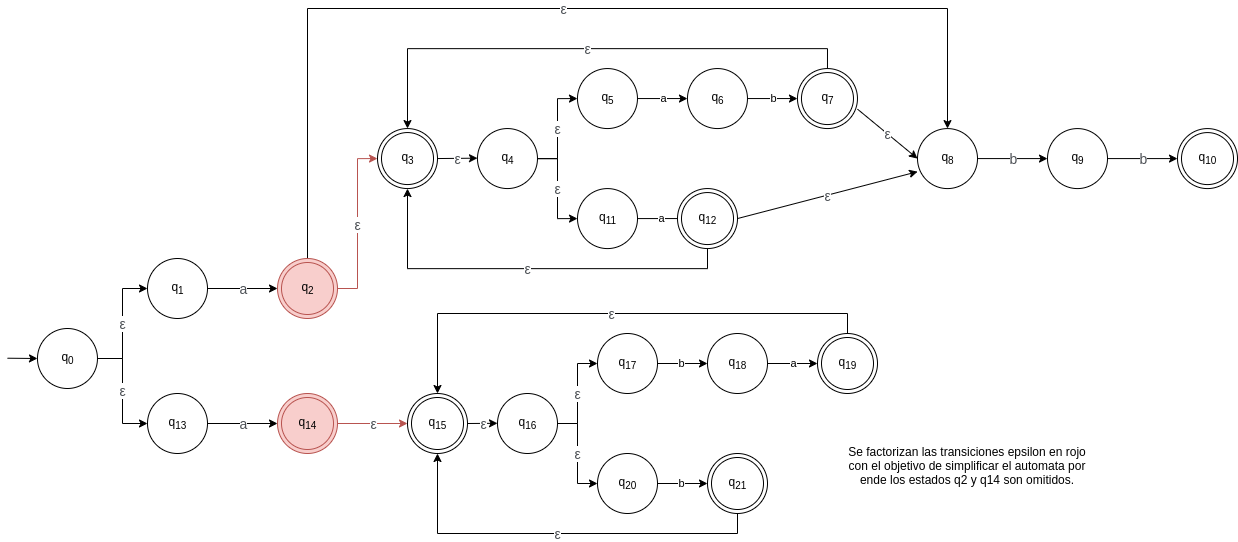
\includegraphics[scale=0.40]{eliminado.png}
        El automata que queda tras la sintesis es...
        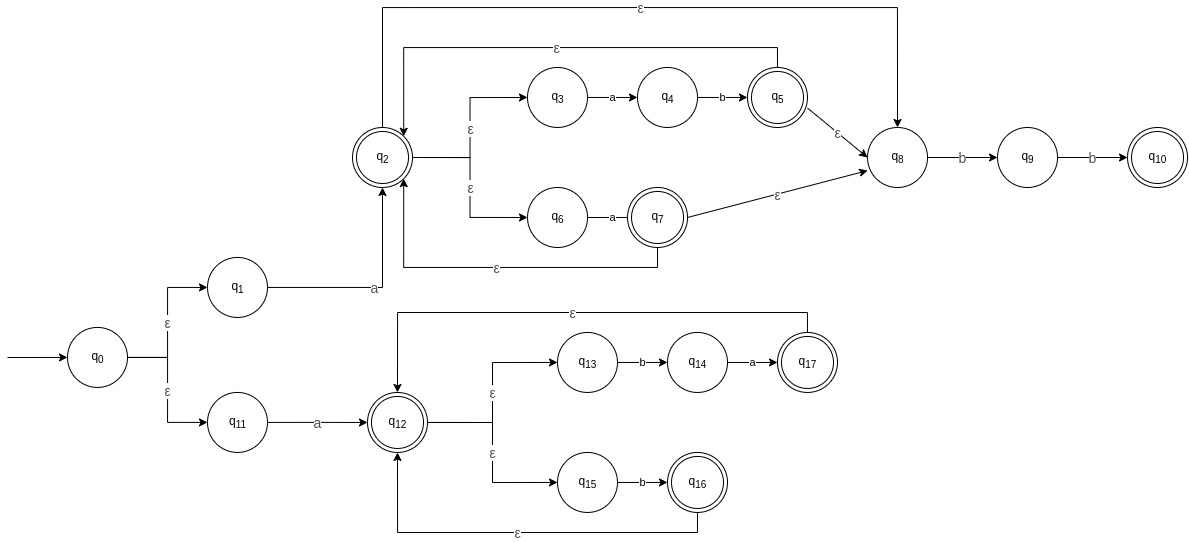
\includegraphics[scale=0.40]{elBueno.png}
    \end{center}

    \item Calcular el conjunto $Cl_{\epsilon}$(q) para cada estado q de la m\'aquina.
    \begin{center}
        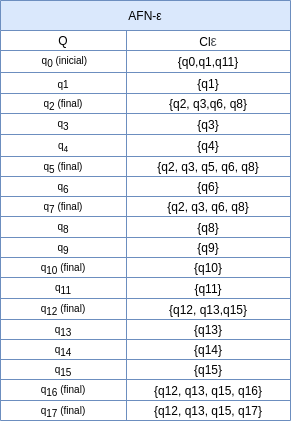
\includegraphics[scale=0.40]{tableTransition.png}
    \end{center}
    \item Encontrar el AFN equivalente a M.
    \begin{center}
        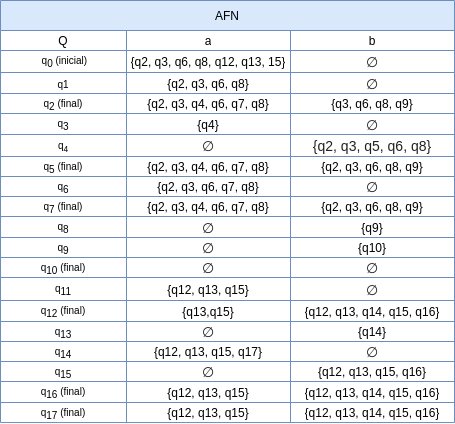
\includegraphics[scale=0.40]{secondTableexam3.png}    
    \end{center}
    
    \item Transformar a un AFD equivalente.
    \item Encontrar el AFD m\'inimo equivalente.        
\end{enumerate}

\question \textbf{2.5pts.} Encuentra una expresi\'on regular $\alpha$ tal que L(M) = L($\alpha$) para el siguiente
aut\'omata M:
        
\begin{center}
    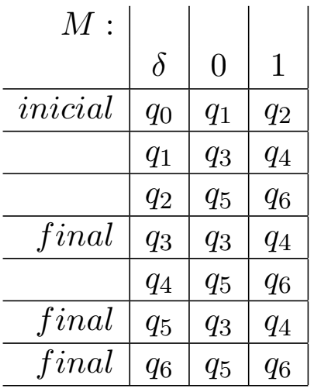
\includegraphics[scale=0.5]{exam2firstTable.png}
\end{center}
 Para clarificar el automata lo transformare a un AFD
\begin{center}
    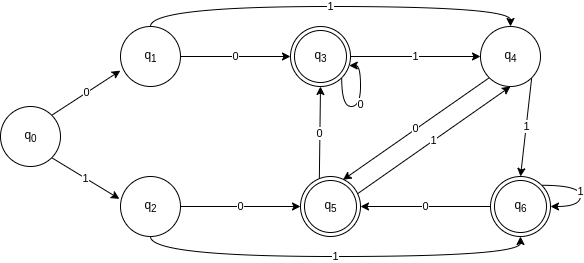
\includegraphics[scale=0.5]{secondQuestion.png}
    \\
    Ejemplos de cadenas: \\

    \textbf{Aceptadas:} \\
    11 \\
    1111111111111 \\
    00 \\
    0010 \\
    0010000010 \\
    0011 \\
    00000000 \\ 
    \textbf{No aceptadas:} \\
    0\textbf{01} \\
    \textbf{01} \\
    010\textbf{01} \\
    11\textbf{01} \\
\end{center}
Ya que es claro que las no aceptadas terminan con \textbf{01} agregaremos la condici\'on 
de que las cadenas tienen que terminar en (11 + 0) para no aceptar ese caso. \\
Tambien notaremos que la longitud de las cadenas no parece importar por ende para llenar el cuerpo
escribiremos (a + b)*, por \'ultimo el automata denota que al inicio tiene que haber al menos 
un 1 o un 0 por ende agregaremos al inicio la condicion (1 + 0).Tambien agregu\'e un + para tambien 
poder aceptar la cadena 11
\\
La expresion regular que describe el automata es:
\begin{equation}
    \alpha = (1 + 0)^{*}(11 + 0)
\end{equation}

\question \textbf{Hasta 1pt extra.} Minimiza el aut\'omata del ejercicio2.